\documentclass[tikz,border=10pt]{standalone}
\usepackage{tikz}
\usepackage{pgfplots}
\usetikzlibrary{patterns,decorations.pathmorphing}

\begin{document}
    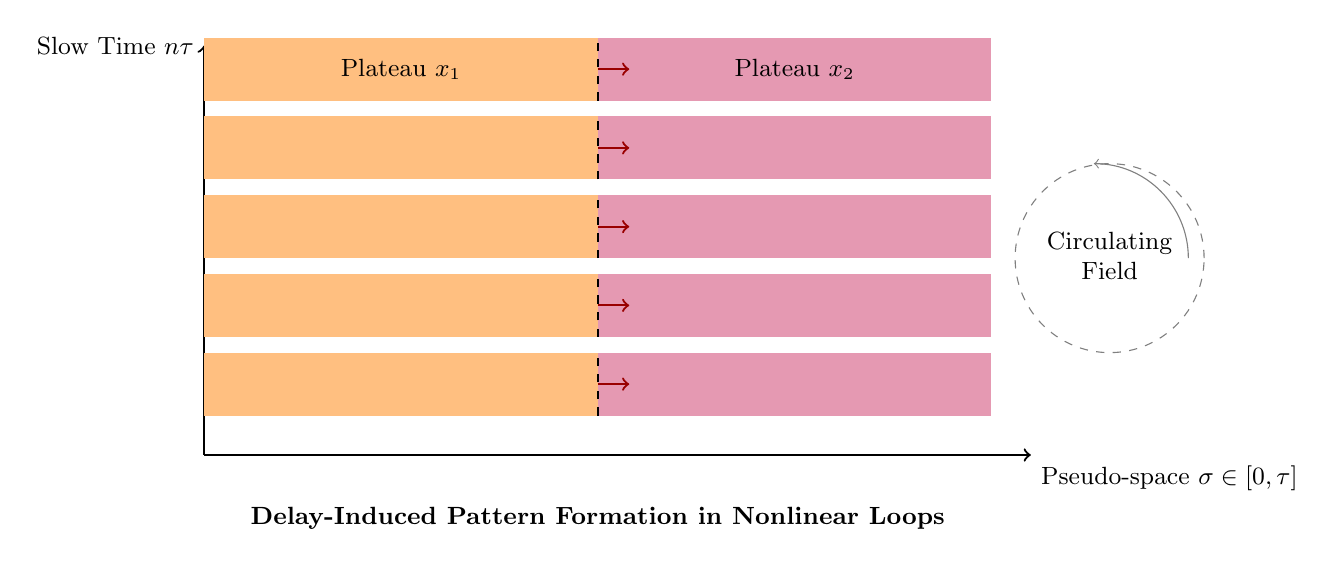
\begin{tikzpicture}

% Axes
        \draw[->, thick] (0,0) -- (0,5.2) node[left] {\small Slow Time $n\tau$};
        \draw[->, thick] (0,0) -- (10.5,0) node[below right] {\small Pseudo-space $\sigma \in [0,\tau]$};

% Plateaus and Fronts
        \foreach \y in {0.5,1.5,...,4.5} {
            \fill[orange!50] (0,\y) rectangle (5,\y+0.8);
            \fill[purple!40] (5,\y) rectangle (10,\y+0.8);
            \draw[dashed, thick] (5,\y) -- (5,\y+0.8); % domain wall
        }

% Labeling plateaus
        \node at (2.5,4.9) {\small Plateau $x_1$};
        \node at (7.5,4.9) {\small Plateau $x_2$};

% Front arrows
        \foreach \y in {0.5,1.5,...,4.5} {
            \draw[->, thick, red!60!black] (5,\y+0.4) -- (5.4,\y+0.4);
        }

% Loop circle sketch (optional visual)
        \draw[dashed, gray] (11.5,2.5) circle(1.2);
        \node at (11.5,2.5) {\small \begin{tabular}{c}Circulating\\Field\end{tabular}};
        \draw[->, gray] (12.5,2.5) arc[start angle=0,end angle=90,radius=1.2];

% Title
        \node[align=center] at (5,-0.8) {\small \textbf{Delay-Induced Pattern Formation in Nonlinear Loops}};
    \end{tikzpicture}
\end{document}